\section{Hardware Systemarkitektur}
Dette afsnit beskriver arkitektur for hardware i Autogreen.

Forsyning til alle blokke er beskrevet på BDD for system, Figur \ref{fig:bdd_system}. Forsyninger er ikke tegnet ind på øvrige diagrammer for overskuelighedens skyld. Det gælder desuden at alle blokke har fælles reference (GND). 

\clearpage

\subsection{BDD for System}
\begin{figure}[h]
\centering 
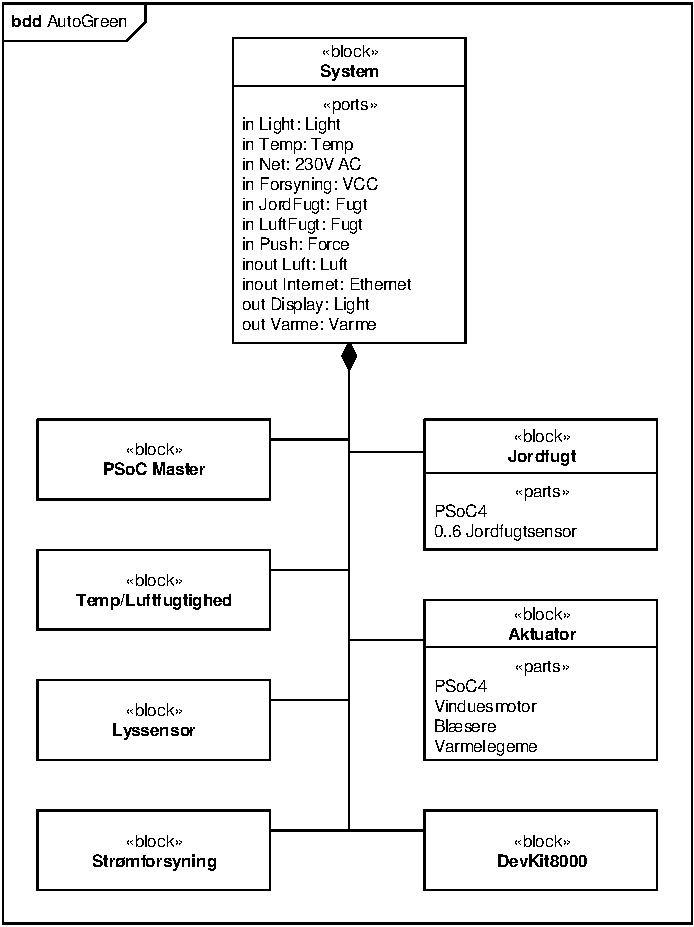
\includegraphics[width={\textwidth-2cm}, trim=0 0 0 0, clip=true] {../fig/bdd_system.pdf}
\caption{BDD for System}
\label{fig:bdd_system}
\end{figure}
\clearpage

\subsection{IBD for System}
%TODO Evt, in out signaler til omverdenen
\begin{figure}[h]
\centering 
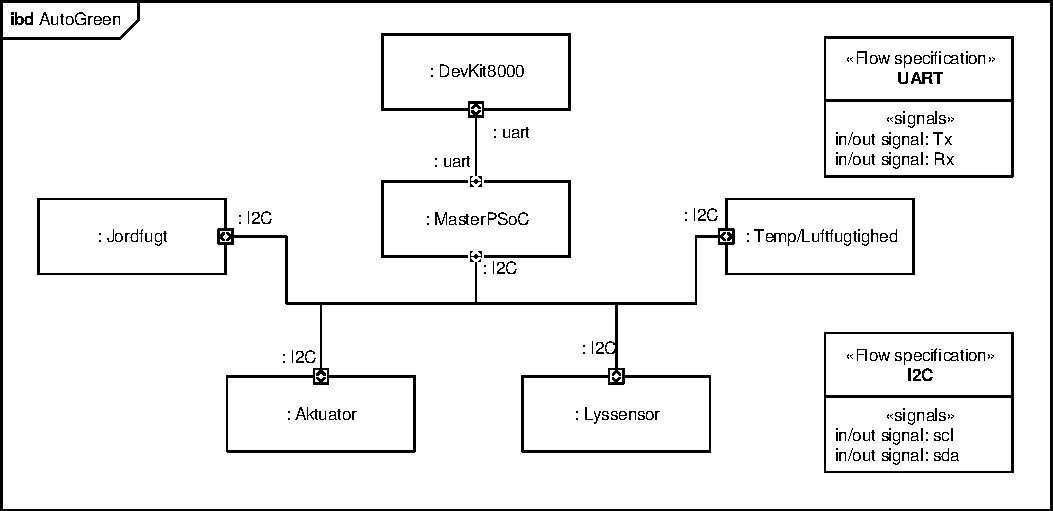
\includegraphics[width={\textwidth}, trim=0 0 0 0, clip=true] {../fig/ibd_system.pdf}
\caption{IBD for System}
\label{fig:ibd_system}
\end{figure}

\subsubsection{Strømforsyning}
Denne blok forsyner øvrig hardware i systemet, undtagen varmelegemet. Blokken forsynes fra en laboratorieforyning. 
\subsubsection{DevKit8000}
Denne blok indeholder systemets brugerflade, og er kontroller for systemet. 
\subsubsection{MasterPSoC}
Denne blok indeholder et PSoC4 Pioneer Kit, der har til opgave at kommunikere via UART med DevKit8000 og via \IIC med slaver.  
\subsubsection{Temp/Luftfugtighed}
Denne blok indeholder en sensor med \IIC interface, og måler temperatur og luftfugtighed i det fysiske drivhus.
\subsubsection{Lyssensor}
Denne blok indeholder en sensor med \IIC interface, og måler lysintensitet i det fysiske drivhus. 
\subsubsection{Jordfugt}
Denne blok indeholder op til seks analoge jordfugtsensorer, som vha. et PSoC4 Pioneer Kit er koblet på systemets \IIC bus.
\subsubsection{Aktuator}
Denne blok indeholder et PSoC4 Pioneer Kit, der fungerer som \IIC slave og styrer systemets aktuatorer. 

\subsection{IBD for Aktuator}

\begin{figure}[h]
\centering 
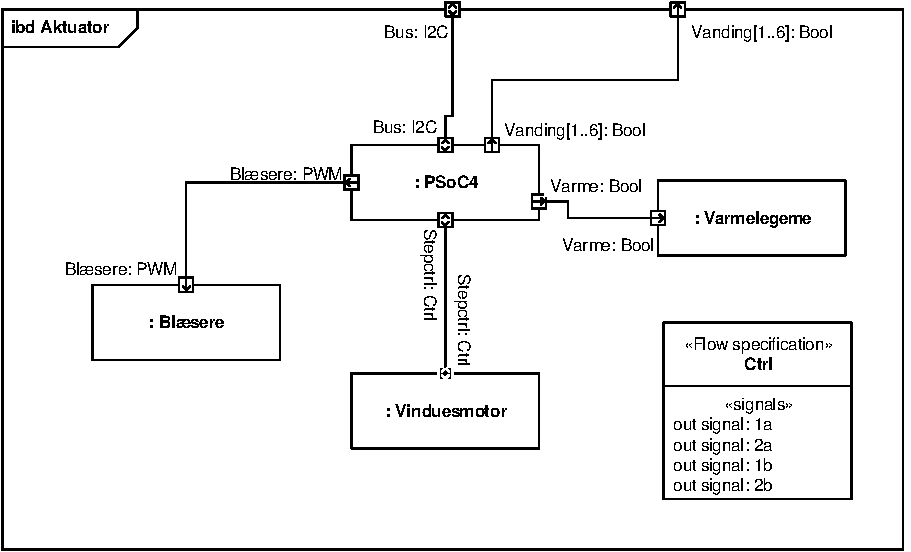
\includegraphics[width={\textwidth}, trim=0 0 0 0, clip=true] {../fig/ibd_aktuator.pdf}
\caption{IBD for Aktuator}
\label{fig:ibd_aktuator}
\end{figure}

\subsubsection{PSoC4}
Denne blok består af et PSoC4 Pioneer Kit, der er \IIC slave. 
\subsubsection{Vinduesmotor}
Denne blok består af en steppermotor, der styrer vinduet i det fysiske drivhus.
\subsubsection{Varmelegeme}
Denne blok består af et varmelegeme, som kan hæve temperaturen i det fysiske drivhus. Varmelegemet styres af PSoC4 blokken, og det forsynes direkte fra elnettet (230V AC). 
\subsubsection{Blæsere}
Denne blok består af nogle blæsere, som kan ventilere luften i det fysiske drivhus. Blæserne styres af PSoC4, og de forsynes fra Strømforsyning. 

\subsection{IBD for Jordfugt}

\begin{figure}[h]
\centering 
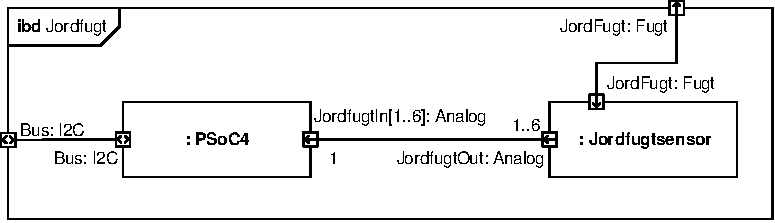
\includegraphics[width={\textwidth}] {../fig/ibd_jordfugt.pdf}
\caption{IBD for Jordfugt}
\label{fig:ibd_jordfugt}
\end{figure}

\subsubsection{PSoC4}
Denne blok består af et PSoC4 Pioneer Kit, der agerer slave på \IIC-bussen. 
\subsubsection{Jordfugtsensor}
Denne blok indeholder en analog sensor, der måler jordfugt ved en plante i det fysiske drivhus. Der kan kobles op til seks af disse til PSoC4.

\clearpage

%TODO lav LTX TBL
\section{Signalbeskrivelser}
\begin{table}[h!]
\centering
\begin{tabularx}{\textwidth}{| l | >{\raggedright}X | >{\raggedright}X | >{\raggedright\arraybackslash}X |>{\raggedright}X |}
\hline
	\textbf{Signaltype} & \textbf{Funktion} & \textbf{Tolerancer} & \textbf{Kommentar}\\ \hline
	VCC & Forsyning til strømforsyning & 12V $\pm$ 0,1V \newline 3A max. & Lab.forsyning  \\\hline	
	VDD & Forsyning til alle PSoC4 Pioneer Kits og DevKit8000. & 5V DC $\pm$ 0.1V, \newline 0.5A max & ~ - \\\hline
	VEE & Forsyning til sensorer & 3.3V DC $\pm$ 0.1V, \newline 0.1A max & ~ - \\\hline
	12V DC Blæsere & Forsyning til blæsere. & 12V DC $\pm$ 0.1V, \newline 140mA max. & - \\\hline	
	12V DC Motor & Forsyning til vinduesmotor. & 12V $\pm$ 0.1V, \newline 500mA max. & - \\\hline
	230V AC & Forsyning til varmelegeme. & 230V AC $\pm$ 10\%, \newline 50 Hz, \newline 0.3A max & - \\\hline
	Analog & Analogt målesignal fra jordfugtmåler. & 0-5V $\pm$ 0.1V & 
	Nivaeuer: \newline
	1: (0.0-0.1)*VEE \newline 
	2: (0.1-0.2)*VEE \newline
	3: (0.2-0.3)*VEE \newline
	4: (0.3-0.4)*VEE \newline
	5: (0.4-0.5)*VEE \newline
	6: (0.5-0.6)*VEE \newline
	7: (0.6-0.7)*VEE \newline
	8: (0.7-0.8)*VEE \newline
	9: (0.8-0.9)*VEE \newline
	10: (0.9-1.0)*VEE \newline	
	Hysterese: 50mV\\\hline		
	Bool & Digitalt signal til styring af vanding og varmelegeme. & 0-3.3V & 1=True: 2.8-3.3V \newline 0=False: 0-0.4V \\\hline	
	Ctrl & Styring af stepper motor & 0-3.3V & 1=True: 2.8-3.3V \newline 0=False: 0-0.4V  \newline Består af fire signaler: \newline 1a, 2a, 1b, 2b \\\hline	
	GND & Stel & 0V & Reference \\\hline	
	I2C & Kommunikation mellem \IIC enheder. & 0-3.3V & 1=True: 2.8-3.3V \newline 0=False: 0-0.4V \newline Består af to signaler: \newline sca og scl \\\hline	
	UART & Kommunikation mellem DevKit8000 og Master & 0-5V & 1=True: 4.5-5V \newline 0=False: 0-0.4V \newline Består af 2 signaler: \newline Tx og Rx \\\hline	
	PWM & Styring af blæsere vha. pulsbreddemodulation. & 0-5V \newline 1 kHz & Dutycycle styres fra 0-100\% i trin fra 0-255. \\\hline	
	\end{tabularx}
\caption{Beskrivelse af signaler.}
\label{tbl:signalbeskriv}
\end{table}

\clearpage